
%%%%%%%%%%%%%%%%%%%%%%%%%%%%%%%%%%%%%%%%%%%%%%%%%%%%%%%%%%%%%%%%%%%%%%%%%%%%%%%%%%%%%%%
%%%%%%%%%%%%%%%%%%%%%%%%%%%%%%%%%%%%%%%%%%%%%%%%%%%%%%%%%%%%%%%%%%%%%%%%%%%%%%%%%%%%%%%
% 
% This top part of the document is called the 'preamble'.  Modify it with caution!
%
% The real document starts below where it says 'The main document starts here'.

\documentclass[12pt]{article}

\usepackage{amssymb,amsmath,amsthm}
\usepackage[top=1in, bottom=1in, left=1.25in, right=1.25in]{geometry}
\usepackage{fancyhdr}
\usepackage{enumerate}
\usepackage{listings}
\usepackage{graphicx}
\usepackage{float}

\usepackage{mwe}
\usepackage{caption}
\usepackage{subcaption}
% Comment the following line to use TeX's default font of Computer Modern.
\usepackage{times,txfonts}



\makeatletter
\renewcommand*\env@matrix[1][*\c@MaxMatrixCols c]{%
  \hskip -\arraycolsep
  \let\@ifnextchar\new@ifnextchar
  \array{#1}}
\makeatother

\newtheoremstyle{homework}% name of the style to be used
  {18pt}% measure of space to leave above the theorem. E.g.: 3pt
  {12pt}% measure of space to leave below the theorem. E.g.: 3pt
  {}% name of font to use in the body of the theorem
  {}% measure of space to indent
  {\bfseries}% name of head font
  {:}% punctuation between head and body
  {2ex}% space after theorem head; " " = normal interword space
  {}% Manually specify head
\theoremstyle{homework} 

% Set up an Exercise environment and a Solution label.
\newtheorem*{exercisecore}{Exercise \@currentlabel}
\newenvironment{exercise}[1]
{\def\@currentlabel{#1}\exercisecore}
{\endexercisecore}

\newcommand{\localhead}[1]{\par\smallskip\noindent\textbf{#1}\nobreak\\}%
\newcommand\solution{\localhead{Solution:}}

%%%%%%%%%%%%%%%%%%%%%%%%%%%%%%%%%%%%%%%%%%%%%%%%%%%%%%%%%%%%%%%%%%%%%%%%
%
% Stuff for getting the name/document date/title across the header
\makeatletter
\RequirePackage{fancyhdr}
\pagestyle{fancy}
\fancyfoot[C]{\ifnum \value{page} > 1\relax\thepage\fi}
\fancyhead[L]{\ifx\@doclabel\@empty\else\@doclabel\fi}
\fancyhead[C]{\ifx\@docdate\@empty\else\@docdate\fi}
\fancyhead[R]{\ifx\@docauthor\@empty\else\@docauthor\fi}
\headheight 15pt

\def\doclabel#1{\gdef\@doclabel{#1}}
\doclabel{Use {\tt\textbackslash doclabel\{MY LABEL\}}.}
\def\docdate#1{\gdef\@docdate{#1}}
\docdate{Use {\tt\textbackslash docdate\{MY DATE\}}.}
\def\docauthor#1{\gdef\@docauthor{#1}}
\docauthor{Use {\tt\textbackslash docauthor\{MY NAME\}}.}
\makeatother

% Shortcuts for blackboard bold number sets (reals, integers, etc.)
\newcommand{\Reals}{\ensuremath{\mathbb R}}
\newcommand{\Nats}{\ensuremath{\mathbb N}}
\newcommand{\Ints}{\ensuremath{\mathbb Z}}
\newcommand{\Rats}{\ensuremath{\mathbb Q}}
\newcommand{\Cplx}{\ensuremath{\mathbb C}}
%% Some equivalents that some people may prefer.
\let\RR\Reals
\let\NN\Nats
\let\II\Ints
\let\CC\Cplx
%%%%%%%%%%%%%%%%%%%%%%%%%%%%%%%%%%%%%%%%%%%%%%%%%%%%%%%%%%%%%%%%%%%%%%%%%%%%%%%%%%%%%%%
%%%%%%%%%%%%%%%%%%%%%%%%%%%%%%%%%%%%%%%%%%%%%%%%%%%%%%%%%%%%%%%%%%%%%%%%%%%%%%%%%%%%%%%
% 
% The main document start here.

% The following commands set up the material that appears in the header.
\doclabel{Stat 461: Homework 4}
\docauthor{Stefano Fochesatto}
\docdate{\today}

\begin{document}

\begin{exercise}{1}Identify any outlying observations in this dataset using
  Mahalanobis distance*.  How can you tell they are outlying
  observations?\\

  \begin{footnotesize}
    \begin{verbatim}
      X <-
      structure(c(0.29, 0.61, 0.3, 0.94, 0.81, 0.88, 0.71, 0.82, 0.88, 
      0.93, 0, 0.12, 0.64, 0.49, 0.18, 0.28, 0.75, 0.82, 0.84, 0.21, 
      0.67, 0.45, 0.79, 0.69, 0.47, 0.23, 0.97, 0.2, 0.88, 0.53, 0.86, 
      0.85, 0.63, 0.43, 0.82, 0.7, 0.33, 0.77, 0.05, 0.8, 0.26, 0.54, 
      0.55, 0.82, 0.99, 0.78, 0.68, 0.73, 0.57, 0.67, 0.06, 0.36, 0.46, 
      0.94, 0.58, 0.98, 0.44, 0.12, 0.53, 0.47, 0.6, 0.41, 0.69, 0.24, 
      0.36, 0.05, 0.82, 0.74, 0.19, 0.77, 0.13, 0.76, 0.31, 0.11, 0.64, 
      0.36, 0.31, 0.26, 0.35, 0.63, 0.92, 0.06, 0.86, 0.52, 0.21, 0.76, 
      0.71, 0.5, 0.37, 0.71, 1.324, 1.46, 0.982, 1.472, 1.772, 1.744, 
      1.082, 1.638, 0.948, 1.9, 0.338, 1.32, 1.214, 1.384, 1.368, 1.198, 
      1.482, 1.654, 1.566, 0.912, 0.44, 0.936, 1.388, 1.696, 1.2, 1.384, 
      1.454, 0.412, 1.446, 1.188, 0.94, 0.51, 0.26, 0.54, 0.11, 0.69, 
      0.72, 0.16, 0.6, 0.91, 0.8, 0.62, 0.93, 0.29, 0.17, 0.54, 0.52, 
      0.37, 0.32, 0.06, 0.94, 0.22, 0.2, 0.68, 0.18, 0.2, 0.09, 0.4, 
      0.9, 0.3), .Dim = c(30L, 5L), .Dimnames = list(NULL, c("x1", 
      "x2", "x3", "x4", "x5")))
    \end{verbatim}
    \end{footnotesize}

    \solution Recall that the Mahalanobis distance is a measure of distance from an observation to the 
    center of the data, de-correlated by the estimated covariance matrix, 
    \begin{equation*}
      D^2 = (\hat{x} - \hat{\mu})^{T}S^{-1}(\hat{x} - \hat{\mu})
    \end{equation*}
    We can quickly compute this distance over all observations $\hat{x}$ using the Mahalanobis() function in r. 
    Doing so we get the following, \\
    \textbf{Code:}
    \begin{center}
    \lstinputlisting[basicstyle = \footnotesize]{r1.txt}
    \end{center}
    \begin{figure}[H]
      \begin{center}
        \caption{Visualizing the $\chi^2$ $95\%$ cutoff.}
      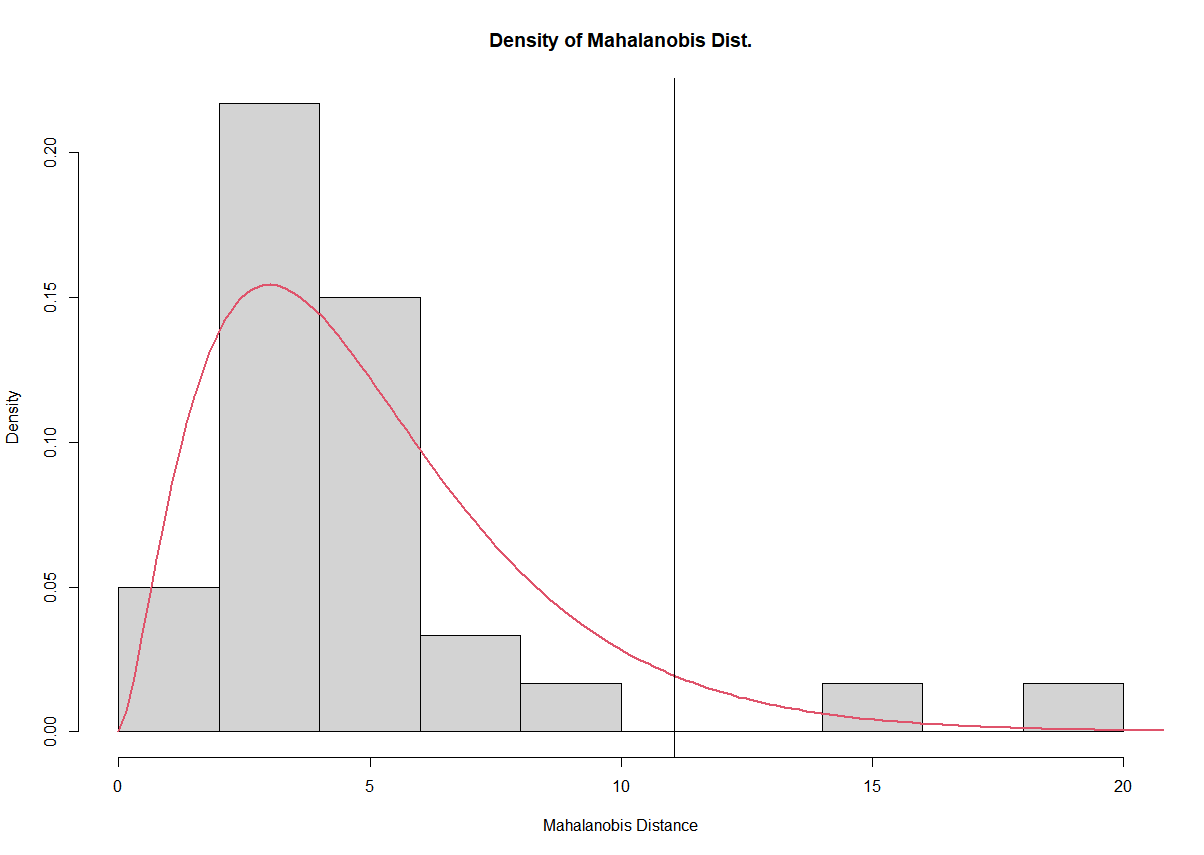
\includegraphics[width = \textwidth]{Rplot10.png}
      \end{center}
    \end{figure}
    \begin{figure}[H]
      \begin{center}
        \caption{Pair Plot with Outliers Highlighted}
      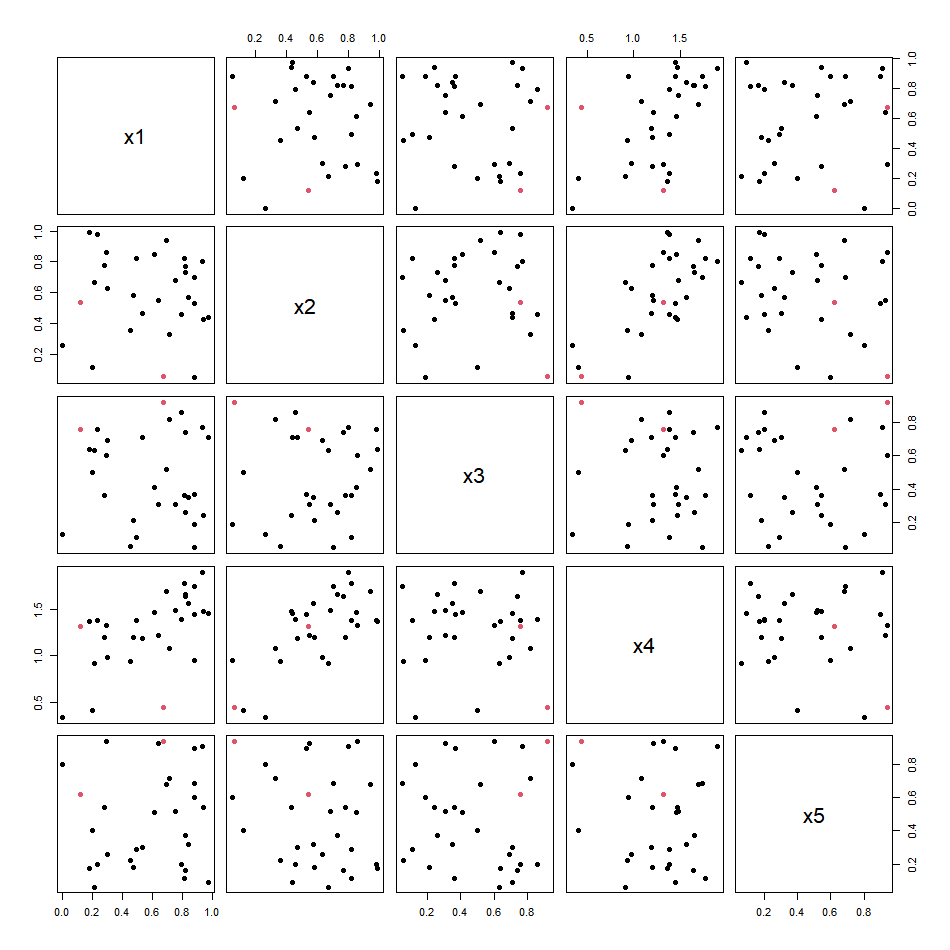
\includegraphics[width = .75\textwidth]{Rplot.png}
      \end{center}
    \end{figure}  
\end{exercise}


\begin{exercise}{2} Beginner's approach to ANOSIM:\\
  \begin{enumerate}
    \item[a] Consider the following observations (species counts):
    \begin{footnotesize}
      \begin{verbatim}
        GROUP  sp1   sp2   sp3   sp4   sp5   sp6   sp7
    
        A      0       0     1     6     1     2    0 
        A      0       4     3     8     3     9    0 
        B      1       1     1     0     0     0    11 
        B      8       3     0     0     0     0    0
      \end{verbatim}
      \end{footnotesize} 
      Compute the Bray-Curtis **dissimilarity** (BC) between each pair of observations and make
      a 4x4 "distance" matrix out of the values, where the entry in the $ith$ row and $jth$ column
      is the Bray-Curtis dissimilarity index between the $ith$ and $jth$ observations, computed as 
      \begin{equation*}
        BC = {{\sum_{s=1}^7 |n_{ik} - n_{jk}|}\over{\sum n_{ik} + n_{jk}}}
      \end{equation*}
      where $n_{ik}$ is the count for the ith observation and kth species. So, for the first two rows, 
      $BC = (0+4+2+2+2+7+0)/(0+4+4+14+4+11+0) = 0.4594$.  This will give the same answer as the approach 
      described in class to compute the Bray-Curtis dissimilarity index.\\
      \solution We can quickly compute the Bray-Curtis dissimilarity index by using the vegdist() function from the vegan package. 
      Doing so we get the following, \\
      \textbf{Code:}
      \begin{center}
      \lstinputlisting[basicstyle = \footnotesize]{r2.txt}
      \end{center}
      \vspace{.15in}




      \item[b] Now replace each "distance" with its rank (shortest distance is
      rank 1, second shortest is 2, etc.).\\
      \solution  Doing so we get the following, 
      \begin{center}
        \begin{tabular}{c|c c c}
           & 1 & 2 & 3 \\
          \hline 
         2 & 1 &   &   \\
         3 & 5 & 4 &   \\
         4 & 6 & 3 & 2 \\
         \end{tabular}
        \end{center}
      \vspace{.15in}




      \item[c] Let rw = average rank within groups A and B. Let rb = average rank between groups A and B\\
      Then the ANOSIM statistic is:
      \begin{equation*}
        R = (rb - rw)/(N*(N-1)/4).
      \end{equation*} 
      ANOSIM is a very robust relative of MANOVA, where we will check to see if two groups are distinct, 
      which we will determine by comparing $R$ to the null distribution of $R$ that we get by permuting the 
      observations (mixing up groups A and B).\\
         \solution Computing rw we get the following, 
         \begin{equation*}
           rw = \dfrac{1 + 2}{2} = \dfrac{3}{2}.
         \end{equation*}
         Computing rb we get the following, 
         \begin{equation*}
           rb = \dfrac{5 + 4 + 6 + 3}{4} = \dfrac{9}{2}.
         \end{equation*}
         Computing the ANOSIM statistic with $N = 4$ for the number of samples. 
         \begin{equation*}
           R = \dfrac{\frac{9}{2} - \frac{3}{2}}{\frac{4*3}{4}} = 1
         \end{equation*} 
         Interpreting this statistic we would say that there is more similarity between observations inside groups than 
         observations outside of the groups. 
      \vspace{.15in}

      \item[d]   BONUS:  Perform a permutation test of Ho:  groups are same vs Ha:
      groups are different, using the ANOSIM statistic.\\
      \solution There are only 2 more permutations possible, which produce a different ANOSIM statistic. The first being 
      one where we swap observation 2 and 3, and the second where we swap observations 2 and 4. Computing the ANOSIM statistic with observations 
      2 and 3 swapped we get the following, 
      \begin{equation*}
        rw = \dfrac{5 + 3}{2} = 4.
      \end{equation*}
      Computing rb we get the following, 
      \begin{equation*}
        rb = \dfrac{1 + 6 + 4 + 2}{4} = \dfrac{13}{4}.
      \end{equation*}
      Computing the ANOSIM statistic with $N = 4$ for the number of samples. 
      \begin{equation*}
        R = \dfrac{\dfrac{13}{4} - 4}{\frac{4*3}{4}} = -.25.
      \end{equation*} 

      Computing the ANOSIM statistic with observations 2 and 4 swapped we get the following, 
      \begin{equation*}
        rw = \dfrac{6 + 4}{2} = 5.
      \end{equation*}
      Computing rb we get the following, 
      \begin{equation*}
        rb = \dfrac{1 + 5 + 3 + 2}{4} = \dfrac{11}{4}.
      \end{equation*}
      Computing the ANOSIM statistic with $N = 4$ for the number of samples. 
      \begin{equation*}
        R = \dfrac{\dfrac{11}{4} - 5}{\frac{4*3}{4}} = -.75.
      \end{equation*} 
      Given that we have so little data I'm not sure how we would approximate the null dist. and compute a worthwhile p-value. I would say that 
      after computing the other permutations, they seem to corroborate the idea that groups are different. Since we got a negative test statistic every time we swapped observations between groups, this 
      implies that there is a greater difference among observations inside groups that across groups. 
  \end{enumerate}
      \vspace{1in}


\begin{exercise}{3}Similarity measures and dissimilarity measures for presence-
  absence data:
  \begin{footnotesize}
    \begin{verbatim}
      obs sp1 sp2 sp3 sp4 sp5 sp6 sp7 sp8 
      1   1   1   1   0   0   0   0   0 
      2   0   0   1   1   1   0   1   0 
      3   0   0   0   0   1   1   1   1
    \end{verbatim}
    \end{footnotesize} 
    
    \begin{enumerate}
      \item[a]  Compute the simple matching index between each pair of
      observations.\\
      \solution Recall that the simple matching index between a pair of observations is the following,
      \begin{equation*}
        s(x_1, x_2) = \dfrac{\text{\# of matching presence} + \text{\# of matching absence}}{\text{\# of predictors}}
      \end{equation*}
      Computing the simple matching index between each pair we get the following, 
      \begin{equation*}
        s(x_1, x_2) = \dfrac{1 + 2}{8} = \dfrac{3}{8}.
      \end{equation*}
      \begin{equation*}
        s(x_1, x_3) = \dfrac{0 + 1}{8} = \dfrac{1}{8}.
      \end{equation*}
      \begin{equation*}
        s(x_2, x_3) = \dfrac{2 + 2}{8} = \dfrac{1}{2}.
      \end{equation*}
      \vspace{.15in}



      \item[b] Compute the Dice-Sorensen index between each pair of observations.\\
      \solution Recall that the Dice-Sorensen index is computed by the following, 
      \begin{equation*}
        s(x_1, x_2) = \dfrac{2*\text{\# of matching presence}} {2*\text{\# of matching presence} + \text{\# only presence in $x_1$} + \text{\# only presence in $x_2$}}
      \end{equation*}
      Computing the Dice-Sorensen index for between each pair of observations we get the following, 
      \begin{equation*}
        s(x_1, x_2) = \dfrac{2(1)}{2(1) + 2 + 3} = \dfrac{2}{7}.
      \end{equation*}
      \begin{equation*}
        s(x_1, x_3) = \dfrac{2(0)}{2(0)+\dots} = 0.
      \end{equation*}
      \begin{equation*}
        s(x_2, x_3) = \dfrac{2(2)}{2(2) + 2 + 2} = \dfrac{1}{2}.
      \end{equation*}

      \vspace{.15in}
      
      


      \item[c]  Horseshoe effect. Take the Dice-Sorensen (DS) index and compute $1 - DS$ for each pair 
      of observations. This is a dissimilarity index. The three observations seem to follow a 
      steadily changing species composition. Let $1 - DS_{ij}$ be the distance from observation i to 
      observation j.  Sketch a plot with three points, where the ith and jth points are roughly 
      separated by distance $1 - DS_{ij}$.  Trace a line from the 1st to 2nd point and then on to the 
      3rd point.  Does this form a straight line?  The tendency for these plots to be bent is 
      called the horseshoe effect and will become important later in the class.\\
      \solution Computing the $1 - DS$ dissimilarity index, 
      \begin{equation*}
        1 - s(x_1, x_2) = 1 - \dfrac{2}{7} = \dfrac{5}{7}.
      \end{equation*}
      \begin{equation*}
        1 - s(x_1, x_3) = 1 - 0 = 1.
      \end{equation*}
      \begin{equation*}
        1 - s(x_2, x_3) = 1 - \dfrac{1}{2} = \dfrac{1}{2}.
      \end{equation*}
      I'm a little confused as to how the plot you're describing should be constructed. So I made a geometric construction in geogebra. I started with a circle with radius 1 and center 
      $x_1$ then put $x_3$ on that circle. On $x_3$ I constructed a circle with radius $1/2$ then placed $x_2$ on that circle. On $x_2$ I constructed a circle with radius $5/7$ then moved 
      $x_2$ so that it's circle would intersect $x_1$. Connecting the points in order we do see some sort of $\cap$ or horseshoe.
      \begin{figure}[H]
        \begin{center}
          \caption{$1 - DS$ Horseshoe Plot.}
        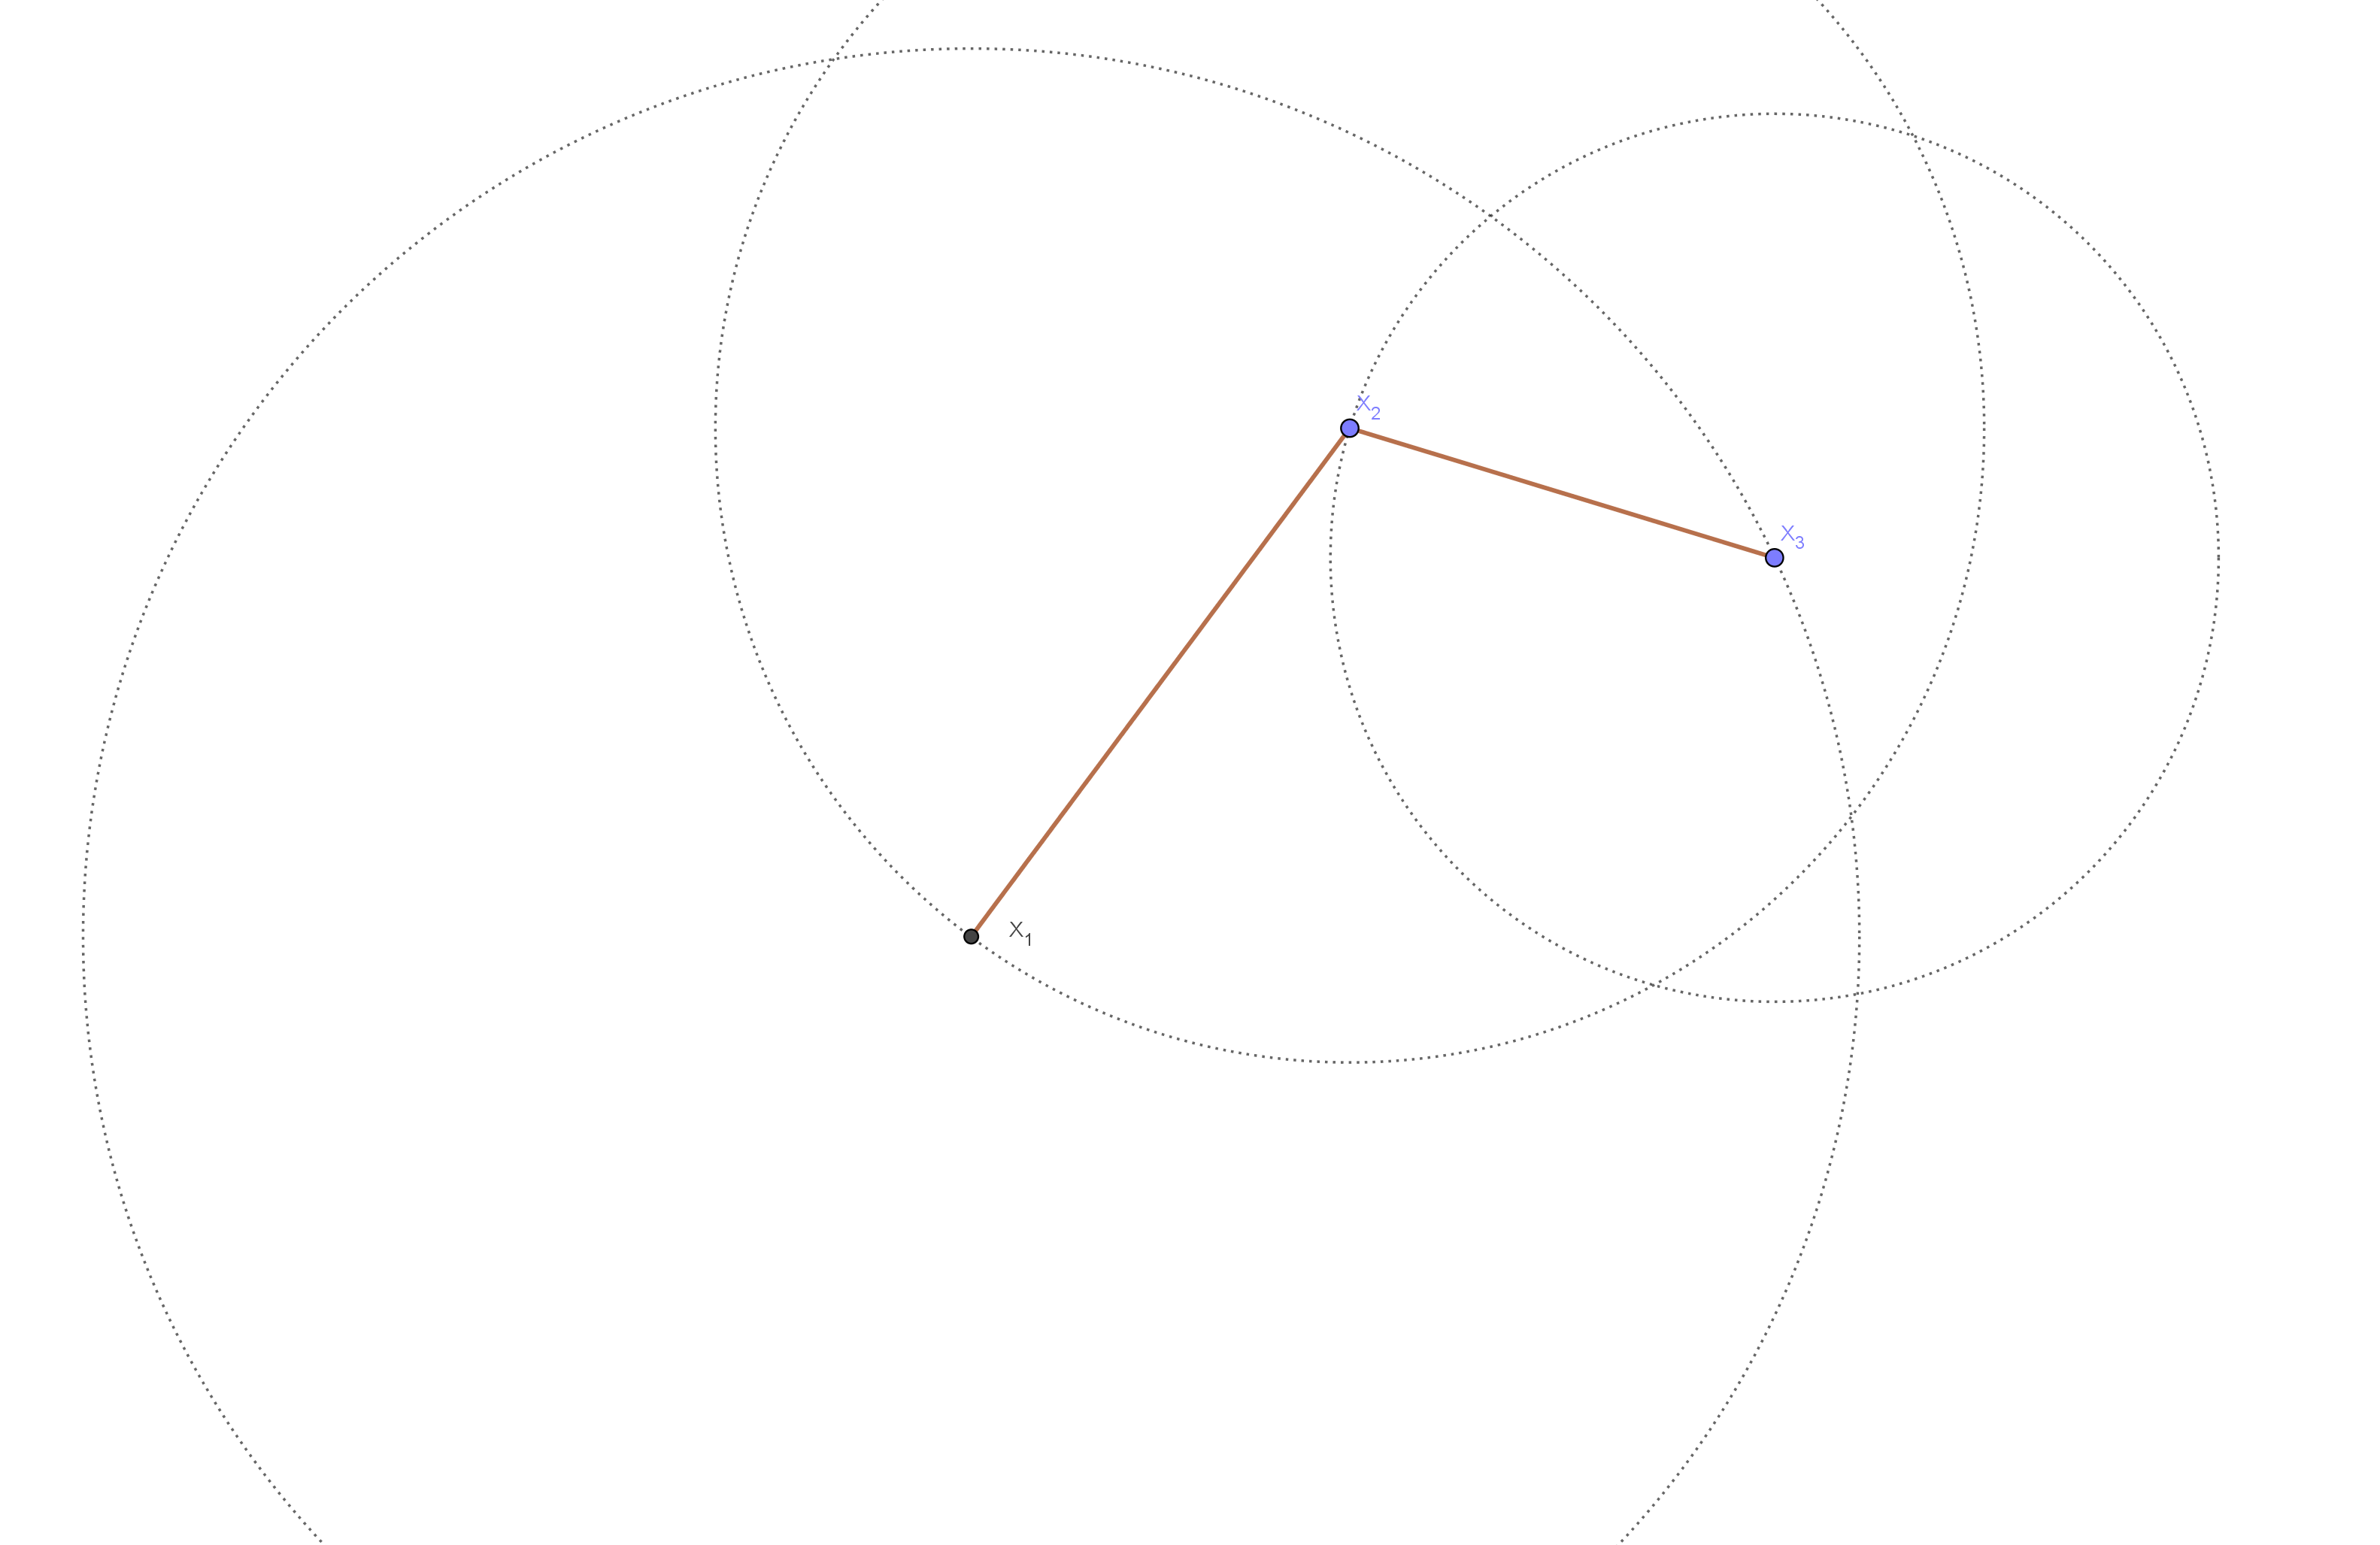
\includegraphics[width = \textwidth]{Horseshoe.png}
        \end{center}
      \end{figure}  
          
    \end{enumerate}
  
\end{exercise}

\vspace{1in}




\begin{exercise}{4} Consider the following set of observations:
  \begin{footnotesize}
    \begin{verbatim}
      obs sp1 sp2 sp3 sp4 
      a   1   0   0   1 
      b   1   1   1   1 
      c   0   1   1   0
    \end{verbatim}
    \end{footnotesize} 
  Find the Dice-Sorensen similarity between each pair, then compute 1 -
  DC as "distances".  Show that 1 - DC isn't really a valid distance, as
  it does not follow the triangle inequality.\\
  \solution Computing the $1 - DC$ dissimilarity index, 
  \begin{equation*}
    1 - s(a, b) = 1 - \dfrac{2(2)}{2(2) + 0 + 2} = \dfrac{1}{3}.
  \end{equation*}
  \begin{equation*}
    1 - s(a, c) = 1 - \dfrac{2(0)}{2(0) + \dots} = 1.
  \end{equation*}
  \begin{equation*}
    1 - s(b, c) = 1 - \dfrac{2(2)}{2(2) + 2 + 0} = \dfrac{1}{3}.
  \end{equation*}
  Recall the triangle equality. If $D$ is a valid distance measure for the observations $a, b, c$ then it must follow that, 
  \begin{equation*}
    D(a,c)\leq D(a,b) + D(b,c).
  \end{equation*}
  Considering $1 - DC$ as a distance measure we get, 
  \begin{equation*}
    1 \leq \dfrac{1}{3} + \dfrac{1}{3}
  \end{equation*}
  Which clearly does not follow the triangle inequality. 
  
\end{exercise}      
\vspace{1in}





\begin{exercise}{5} Consider one of the following 'distance' measures: $1 - (simple matching index)$, $1 - (Dice-Sorensen)$,
  or $1 - (Jaccard)$.  (They are really dissimilarity measures).\\
  \begin{enumerate}
    \item[a]  Does the one you chose to test have the property that
    if the distance between observations is ZERO, then the observations
    have to have exactly the same species composition?\\
    \solution For this problem we will consider the following dissimilarity measure $1 - (simple matching index)$. Recall that for two observations we it 
    is computed by the following, 
    \begin{equation*}
      s(x_1, x_2) = 1 - \dfrac{\text{\# of matching presence} + \text{\# of matching absence}}{\text{\# of predictors}}
    \end{equation*}
    To prove that $1 - (simple matching index)$ has the property that if the distance between observations is ZERO, then the observations
    have to have exactly the same species composition we will use contradiction. Consider two observations $x_1$ and $x_2$ with different species compositions such that 
    $s(x_1, x_2) = 0$. Recall the formula for the $1 - (simple matching index)$ dissimilarity measure,
    \begin{equation*}
      s(x_1, x_2) = 1 - \dfrac{\text{\# of matching presence} + \text{\# of matching absence}}{\text{\# of predictors}} = 0
    \end{equation*} 
    Note that in order for this computation to result in $s(x_1, x_2) = 0$ it follows that, 
    \begin{equation*}
      \text{\# of matching presence} + \text{\# of matching absence} = \text{\# of predictors}
    \end{equation*}
    Clearly this is a contradiction since $x_1$ and $x_2$ with different species compositions so there must be at least one predictor where the observations do not match.     
    \vspace{.15in}




    \item[b] Does the one you chose have the property that if observations are identical (same species composition), then they are distance zero apart?
    \solution Suppose two observations $x_1$ and $x_2$ with the same species compositions, therefore everywhere we have a presence in one observations the other observation must have the same presence, 
    and similarly with absences. Thus we can make the following observation,     
    \begin{equation*}
      \text{\# of matching presence} + \text{\# of matching absence} = \text{\# of predictors}
    \end{equation*}
    As described in the previous section, it follows from here that the dissimilarity index  $1 - (simple matching index)$ will be zero. 
  
  \end{enumerate}
\end{exercise}
 






























\end{exercise}
















\end{document}


















